\chapter{Conclusão}

Fringilla urna porttitor rhoncus dolor. Iaculis urna id volutpat lacus laoreet. Nullam non nisi est sit amet facilisis magna etiam. Ultrices vitae auctor eu augue. Cursus vitae congue mauris rhoncus aenean vel. Donec ultrices tincidunt arcu non. Id diam vel quam elementum pulvinar etiam non quam. Faucibus a pellentesque sit amet porttitor eget dolor. Tellus at urna condimentum mattis pellentesque. Ut sem viverra aliquet eget sit amet tellus cras adipiscing.

\section{Arquitetura do Projeto}

O sistema desenvolvido é composto por uma arquitetura modular integrada em uma plataforma móvel terrestre, com possibilidade de migração para plataforma aérea. A arquitetura pode ser descrita conforme a sequência de transformação de dados:

\begin{center}
LiDAR (sensor) $\rightarrow$ Corpo (drone) $\rightarrow$ Referencial Global
\end{center}

\subsection{Componentes Principais}

O sistema integra três sensores principais para aquisição de dados espaciais:

\begin{itemize}
    \item \textbf{Sensor LiDAR LD06:} Responsável pela medição de distância e ângulo, fornecendo pares (ângulo, distância) com resolução angular e intensidade do retorno, permitindo a geração da nuvem de pontos em 2D.
    
    \item \textbf{Unidades de Medição Inercial (IMU) — 2x MPU-6050:} Medem aceleração em três eixos (ax, ay, az) e velocidade angular (gx, gy, gz), viabilizando a estimação de atitude do drone e a derivação de posição inercial através de integrações sucessivas.
    
    \item \textbf{Microcontrolador Raspberry Pi Pico (RP2040):} Orquestra a leitura dos sensores, sincroniza os dados, aplica filtros de qualidade e registra o conjunto completo em cartão SD. Possui 264 KB de RAM, 2 MB de Flash e periféricos suficientes (2x UART, 2x I2C, 2x SPI) para gerenciar todos os sensores simultaneamente.
\end{itemize}

\subsection{Fluxo de Processamento}

O processamento ocorre em etapas sequenciais:

\begin{enumerate}
    \item \textbf{Aquisição:} Leitura simultânea das duas IMUs via I2C e do LiDAR via UART serial.
    \item \textbf{Filtragem:} Aplicação de filtro de intensidade mínima (223) para garantir qualidade dos dados LiDAR.
    \item \textbf{Sincronização Temporal:} Timestamping em microsegundos para correlacionar medições de sensores distintos.
    \item \textbf{Compensação Inercial:} Transformação de acelerações do referencial do corpo para o referencial global utilizando matrizes de rotação baseadas nos ângulos de Euler (roll, pitch, yaw).
    \item \textbf{Integração Numérica:} Cálculo de velocidade e posição pela dupla integração de aceleração (v = $\int$ a dt, s = $\int$ v dt).
    \item \textbf{Armazenamento:} Gravação contínua em cartão SD no formato CSV para posterior processamento e geração de nuvem de pontos.
\end{enumerate}

\subsection{Diagrama de Arquitetura}

\begin{figure}[H]
    \centering
    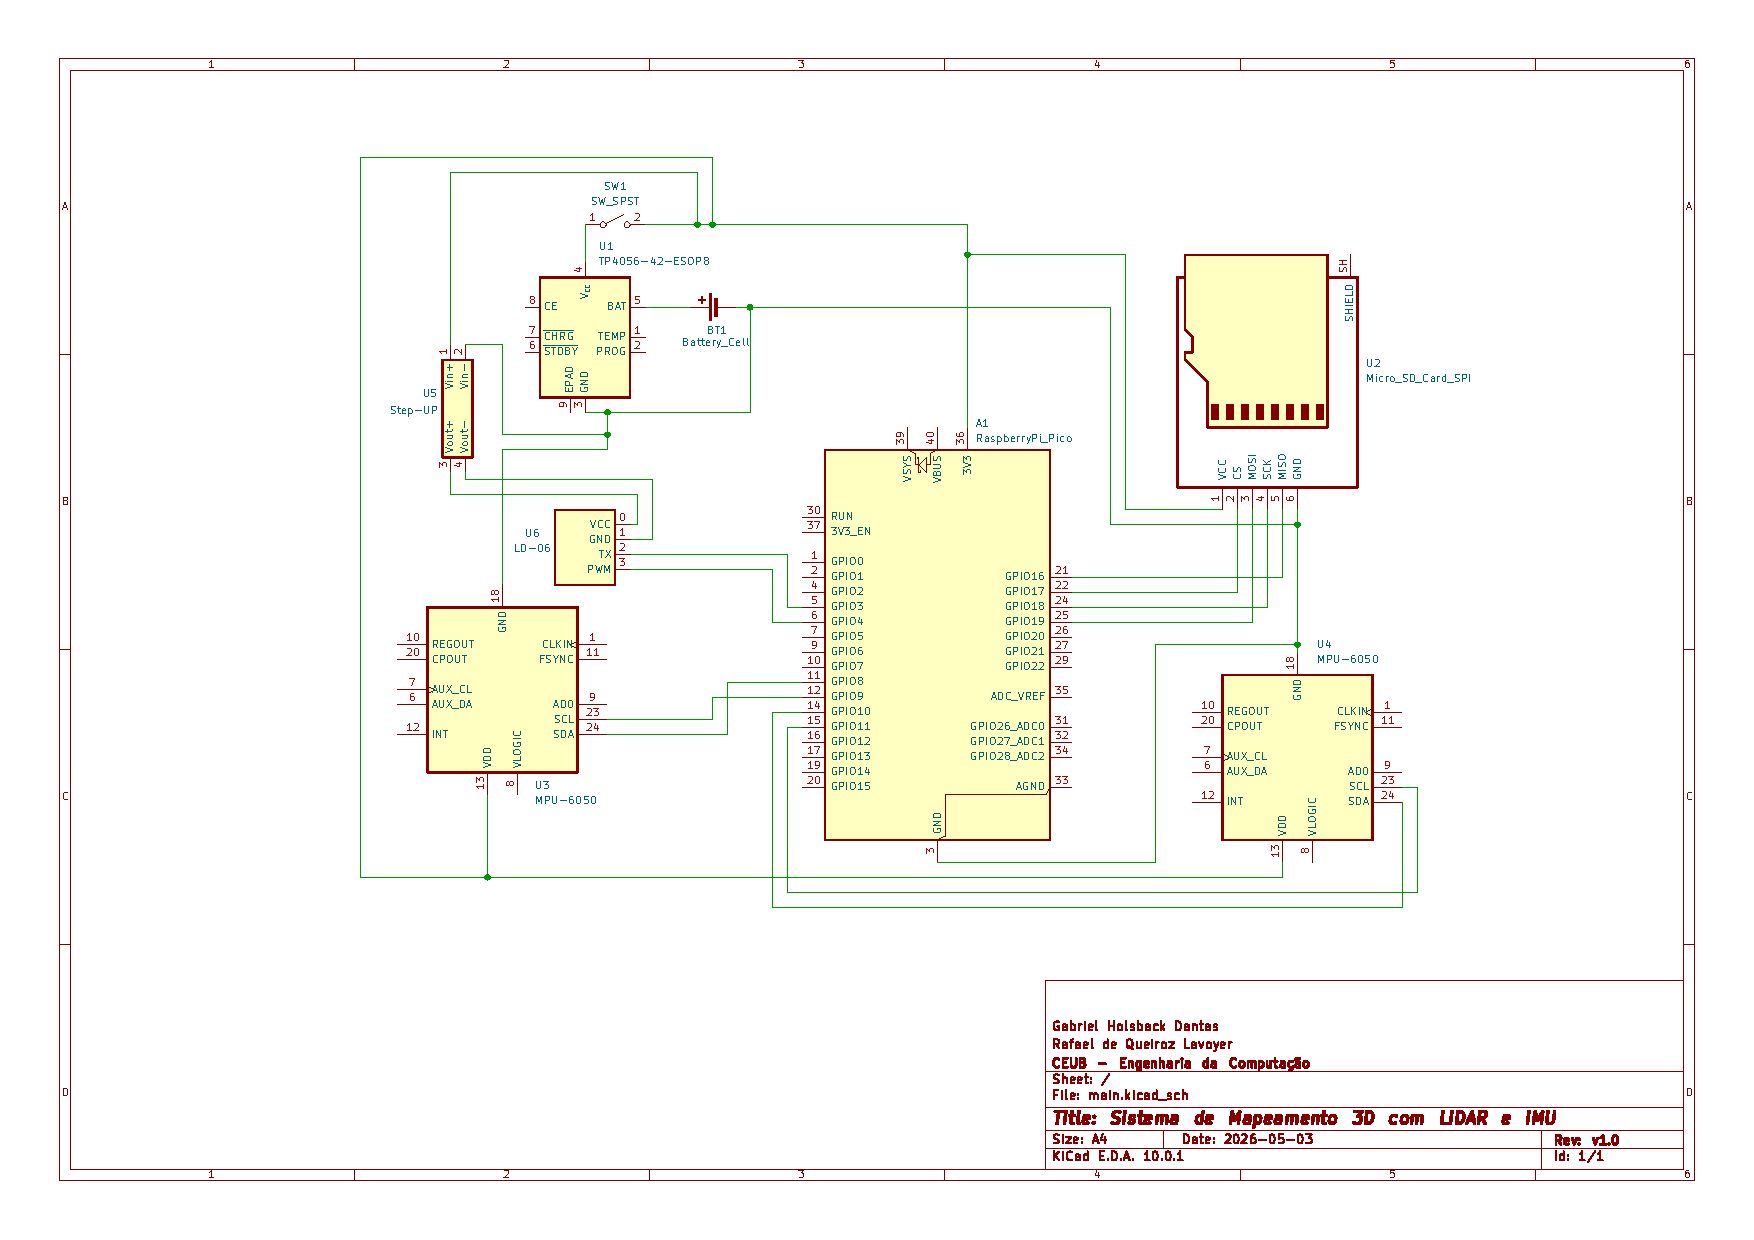
\includegraphics[width=0.8\textwidth]{Componentes}
    \caption{Diagrama esquemático da arquitetura de hardware do sistema de mapeamento 3D, mostrando a integração entre o Raspberry Pi Pico, sensores (LiDAR LD06 e IMUs MPU-6050), módulo de armazenamento (cartão SD) e plataforma móvel.}
    \label{fig:arquitetura_hardware}
\end{figure}

\section{Materiais Utilizados}

O projeto foi implementado com componentes específicos selecionados pela sua adequação aos requisitos de precisão, custo e integração:

\subsection{Componentes Eletrônicos}

\subsubsection{Microcontrolador}
\begin{itemize}
    \item \textbf{Componente:} Raspberry Pi Pico (RP2040)
    \item \textbf{Especificações:} Processador ARM Cortex-M0+ dual-core @ 125 MHz, 264 KB RAM, 2 MB Flash, 2x UART, 2x I2C, 2x SPI, 16x PWM, ADC
    \item \textbf{Função:} Controlar sensores, processar dados e gerenciar armazenamento em tempo real
\end{itemize}

\subsubsection{Sensores Inerciais}
\begin{itemize}
    \item \textbf{Componente:} MPU-6050 (Quantidade: 2 unidades)
    \item \textbf{Especificações:} Acelerómetro ±2g a ±16g, Giroscópio ±250°/s a ±2000°/s, Interface I2C
    \item \textbf{Função:} Medir aceleração (ax, ay, az) e velocidade angular (gx, gy, gz) para estimativa de atitude e posição inercial
\end{itemize}

\subsubsection{Sensor de Distância e Ângulo}
\begin{itemize}
    \item \textbf{Componente:} LiDAR LD06 (2D)
    \item \textbf{Especificações:} UART 230400 baud, Pacotes de 47 bytes com 12 pontos cada, Varredura 0° a 360°, Filtro de qualidade em intensidade ≥ 223
    \item \textbf{Função:} Medir distância e ângulo para geração de nuvem de pontos 2D
\end{itemize}

\subsubsection{Armazenamento}
\begin{itemize}
    \item \textbf{Componente:} Módulo Cartão SD
    \item \textbf{Especificações:} Interface SPI, Capacidade mínima de 16 GB
    \item \textbf{Função:} Registrar 15 variáveis de dados por ciclo em formato CSV
\end{itemize}

\subsection{Dados Coletados}

O sistema coleta um conjunto robusto de dados em cada ciclo de leitura:

\begin{table}[H]
    \centering
    \caption{Estrutura de dados coletados por ciclo}
    \begin{tabularx}{\textwidth}{l|l|X}
        \hline
        \textbf{Variável} & \textbf{Fonte} & \textbf{Descrição} \\
        \hline
        tempo\_us & Relógio & Timestamp em microsegundos \\
        ax1, ay1, az1 & IMU 1 & Aceleração nos 3 eixos (IMU 1) \\
        gx1, gy1, gz1 & IMU 1 & Velocidade angular nos 3 eixos (IMU 1) \\
        ax2, ay2, az2 & IMU 2 & Aceleração nos 3 eixos (IMU 2) \\
        gx2, gy2, gz2 & IMU 2 & Velocidade angular nos 3 eixos (IMU 2) \\
        angle & LiDAR & Ângulo da varredura LiDAR (0° a 360°) \\
        distance & LiDAR & Distância medida (unidades de 0.25 mm) \\
        intensity & LiDAR & Intensidade do retorno laser (0--255) \\
        \hline
    \end{tabularx}
    \label{tab:dados_coletados}
\end{table}

Os dados são armazenados em formato CSV, permitindo análise posterior e processamento para geração da nuvem de pontos com transformação completa de coordenadas.

\section{Dificuldades}

\section{Resultados obtidos}

\subsection{Interpretação dos resultados}

\section{Trabalhos futuros}

\subsection{Comunicação com o drone em cavernas}

\subsection{Navegação autônoma com os dados obtidos}


